\documentclass[12pt,a4paper]{article}

%\usepackage[left=1.5cm,right=1.5cm,top=1cm,bottom=2cm]{geometry}
\usepackage[in, plain]{fullpage}
\usepackage{array}
\usepackage{../../../pas-math}
\usepackage{../../../moncours}


%\usepackage{pas-cours}
%-------------------------------------------------------------------------------
%          -Packages nécessaires pour écrire en Français et en UTF8-
%-------------------------------------------------------------------------------
\usepackage[utf8]{inputenc}
\usepackage[frenchb]{babel}
\usepackage[T1]{fontenc}
\usepackage{lmodern}
\usepackage{textcomp}



%-------------------------------------------------------------------------------

%-------------------------------------------------------------------------------
%                          -Outils de mise en forme-
%-------------------------------------------------------------------------------
\usepackage{hyperref}
\hypersetup{pdfstartview=XYZ}
%\usepackage{enumerate}
\usepackage{graphicx}
\usepackage{multicol}
\usepackage{tabularx}
\usepackage{multirow}


\usepackage{anysize} %%pour pouvoir mettre les marges qu'on veut
%\marginsize{2.5cm}{2.5cm}{2.5cm}{2.5cm}

\usepackage{indentfirst} %%pour que les premier paragraphes soient aussi indentés
\usepackage{verbatim}
\usepackage{enumitem}
\usepackage[usenames,dvipsnames,svgnames,table]{xcolor}

\usepackage{variations}

%-------------------------------------------------------------------------------


%-------------------------------------------------------------------------------
%                  -Nécessaires pour écrire des mathématiques-
%-------------------------------------------------------------------------------
\usepackage{amsfonts}
\usepackage{amssymb}
\usepackage{amsmath}
\usepackage{amsthm}
\usepackage{tikz}
\usepackage{xlop}
%-------------------------------------------------------------------------------



%-------------------------------------------------------------------------------


%-------------------------------------------------------------------------------
%                    - Mise en forme avancée
%-------------------------------------------------------------------------------

\usepackage{ifthen}
\usepackage{ifmtarg}


\newcommand{\ifTrue}[2]{\ifthenelse{\equal{#1}{true}}{#2}{$\qquad \qquad$}}

%-------------------------------------------------------------------------------

%-------------------------------------------------------------------------------
%                     -Mise en forme d'exercices-
%-------------------------------------------------------------------------------
%\newtheoremstyle{exostyle}
%{\topsep}% espace avant
%{\topsep}% espace apres
%{}% Police utilisee par le style de thm
%{}% Indentation (vide = aucune, \parindent = indentation paragraphe)
%{\bfseries}% Police du titre de thm
%{.}% Signe de ponctuation apres le titre du thm
%{ }% Espace apres le titre du thm (\newline = linebreak)
%{\thmname{#1}\thmnumber{ #2}\thmnote{. \normalfont{\textit{#3}}}}% composants du titre du thm : \thmname = nom du thm, \thmnumber = numéro du thm, \thmnote = sous-titre du thm

%\theoremstyle{exostyle}
%\newtheorem{exercice}{Exercice}
%
%\newenvironment{questions}{
%\begin{enumerate}[\hspace{12pt}\bfseries\itshape a.]}{\end{enumerate}
%} %mettre un 1 à la place du a si on veut des numéros au lieu de lettres pour les questions 
%-------------------------------------------------------------------------------

%-------------------------------------------------------------------------------
%                    - Mise en forme de tableaux -
%-------------------------------------------------------------------------------

\renewcommand{\arraystretch}{1.7}

\setlength{\tabcolsep}{1.2cm}

%-------------------------------------------------------------------------------



%-------------------------------------------------------------------------------
%                    - Racourcis d'écriture -
%-------------------------------------------------------------------------------

% Angles orientés (couples de vecteurs)
\newcommand{\aopp}[2]{(\vec{#1}, \vec{#2})} %Les deuc vecteurs sont positifs
\newcommand{\aopn}[2]{(\vec{#1}, -\vec{#2})} %Le second vecteur est négatif
\newcommand{\aonp}[2]{(-\vec{#1}, \vec{#2})} %Le premier vecteur est négatif
\newcommand{\aonn}[2]{(-\vec{#1}, -\vec{#2})} %Les deux vecteurs sont négatifs

%Ensembles mathématiques
\newcommand{\naturels}{\mathbb{N}} %Nombres naturels
\newcommand{\relatifs}{\mathbb{Z}} %Nombres relatifs
\newcommand{\rationnels}{\mathbb{Q}} %Nombres rationnels
\newcommand{\reels}{\mathbb{R}} %Nombres réels
\newcommand{\complexes}{\mathbb{C}} %Nombres complexes


%Intégration des parenthèses aux cosinus
\newcommand{\cosP}[1]{\cos\left(#1\right)}
\newcommand{\sinP}[1]{\sin\left(#1\right)}


%Probas stats
\newcommand{\stat}{statistique}
\newcommand{\stats}{statistiques}
%-------------------------------------------------------------------------------

%-------------------------------------------------------------------------------
%                    - Mise en page -
%-------------------------------------------------------------------------------

\newcommand{\twoCol}[1]{\begin{multicols}{2}#1\end{multicols}}


\setenumerate[1]{font=\bfseries,label=\textit{\alph*})}
\setenumerate[2]{font=\bfseries,label=\arabic*)}


%-------------------------------------------------------------------------------
%                    - Elements cours -
%-------------------------------------------------------------------------------





%\makeatletter
%\renewcommand*{\@seccntformat}[1]{\csname the#1\endcsname\hspace{0.1cm}}
%\makeatother


%\author{Olivier FINOT}
\date{}
\title{}

%\newcommand{\disp}{false}

%\lhead{CH1 : Stats et représentations graphiques}
%\rhead{O. FINOT}
%
%\rfoot{Page \thepage}
\begin{document}
%\maketitle

\chap[num=5, color=red]{Figures planes}{Olivier FINOT, \today }


%\begin{myobj}
%	Être capable de :
%	\begin{itemize}
%		\item traduire un problème en équation ou en inéquation.
%		\item résoudre une équation.
%		\item résoudre une inéquation.
%		\item évaluer ou critiquer un résultat obtenu
%		\item replacer un résultat dans le contexte du problème.
%	\end{itemize}
%\end{myobj}

\section{Triangle et droites remarquables}

Dans un triangle, les droites remarquables sont les médiatrices, les bissectrices, les médianes et les hauteurs.

\subsection{Médiatrice}

\begin{mydef}	
	Une médiatrice est une droite est \kw{perpendiculaire au milieu} d'un coté.	
\end{mydef}

\begin{myprop}
	
	\begin{multicols}{2}
		Les trois médiatrices d'un triangle sont concourantes en un point O, le \kw{centre du cercle circonscrit} au triangle. 
		
		\begin{center}
			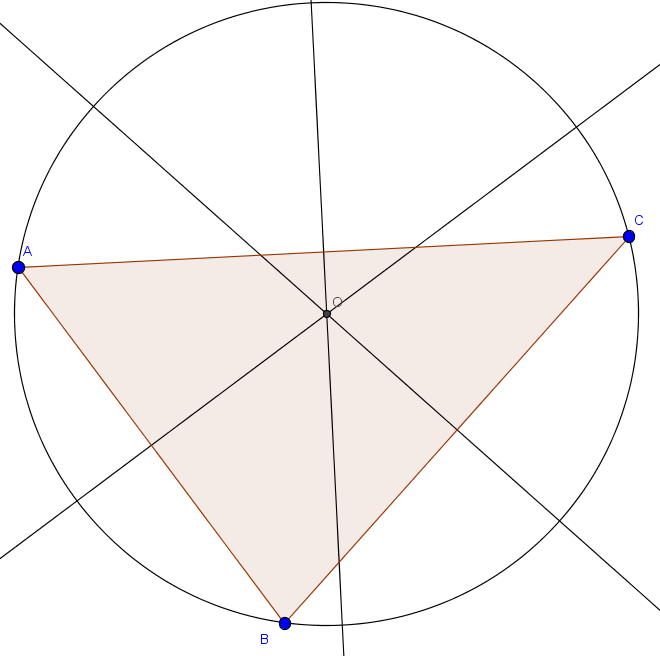
\includegraphics[scale=0.35]{./img/mediatrices}
		\end{center} 
				
	\end{multicols}
\end{myprop}



\subsection{Bissectrice}

\begin{mydef}	
	Une bissectrice est une droite qui \kw{partage un angle en deux angles égaux}.
\end{mydef}

\begin{myprop}
	
	\begin{multicols}{2}
	
		Les trois bissectrices d'un triangle sont concourantes en un point I, le \kw{centre du cercle inscrit} dans le triangle. 

		\begin{center}
			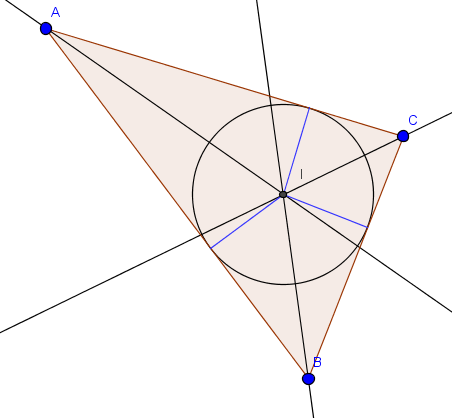
\includegraphics[scale=0.45]{./img/bissectrices}
		\end{center} 
	\end{multicols}
\end{myprop}

\subsection{Médiane}

\begin{mydef}	
	Une médiane est une droite qui passe par le \kw{milieu d'un coté} et par le \kw{sommet opposé}.
\end{mydef}

\begin{myprop}
	
	\begin{multicols}{2}
		
		Les trois médianes d'un triangle sont concourantes en un point G, le \kw{centre de gravité} du triangle. 
		
		\begin{center}
			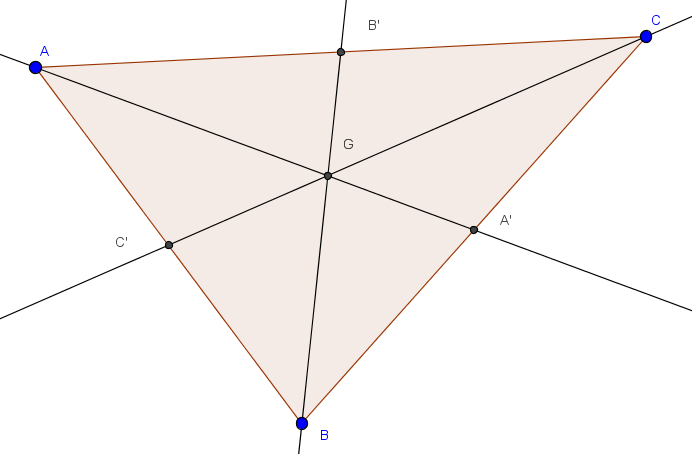
\includegraphics[scale=0.35]{./img/medianes}
		\end{center} 
	\end{multicols}
\end{myprop}

\subsection{Hauteur}

\begin{mydef}	
	Une hauteur est une droite \kw{perpendiculaire à un coté} et qui passe par le \kw{sommet opposé}.
\end{mydef}

\begin{myprop}
	
	\begin{multicols}{2}
		
		Les trois hauteurs d'un triangle sont concourantes en un point H, l' \kw{orthocentre} du triangle. 
		
		\begin{center}
			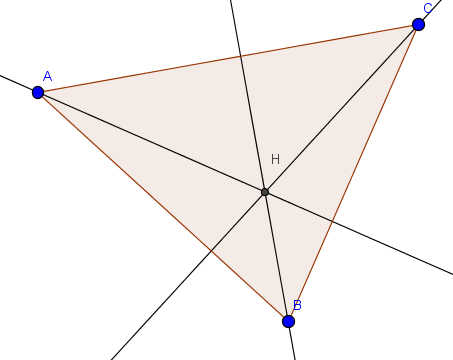
\includegraphics[scale=0.4]{./img/hauteurs}
		\end{center} 
	\end{multicols}
\end{myprop}


\subsection{Aire d'un triangle}

\begin{mymeth}
	\begin{multicols}{2}
		On calcule l'aire d'un triangle en utilisant la formule suivante :
		\kw{\begin{align*}
			Aire &= \dfrac{base \times hauteur}{2} 
		\end{align*}}
		\begin{align*}
			Aire &= \dfrac{AB \times DC}{2}
		\end{align*}
		
		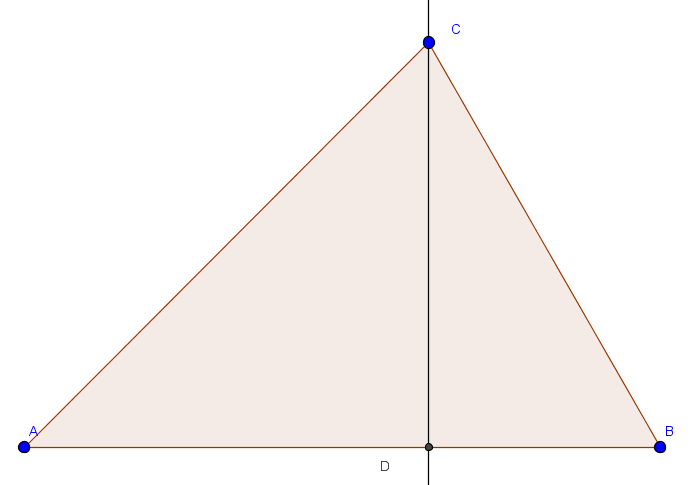
\includegraphics[scale=0.4]{./img/aire-tri}
	\end{multicols}
\end{mymeth}

\section{Quadrilatères et aires}

\subsection{Parallélogramme}

\begin{myprops}
	
	\begin{multicols}{2}

		Dans un parallélogramme :
		\begin{itemize}
			\item Les diagonales se coupent en leur milieu;
			\item Les cotés opposés sont parallèles et égaux.
		\end{itemize}
	
		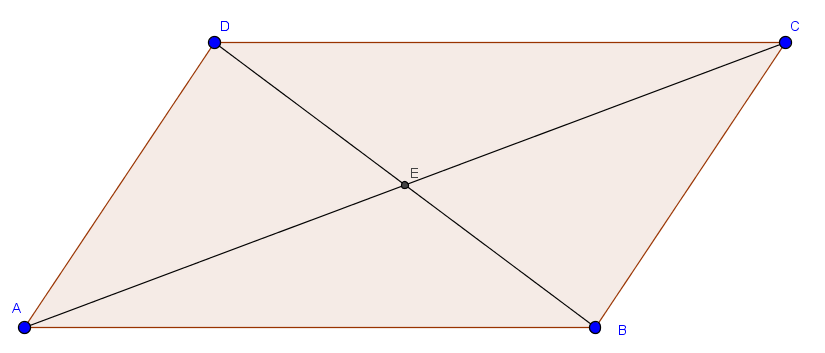
\includegraphics[scale=0.4]{./img/para}
	\end{multicols}
\end{myprops}

\newpage
\subsection{Losange}

\begin{myprops}
	
	\begin{multicols}{2}
		
		Dans un losange :
		\begin{itemize}
			\item Les cotés opposés sont parallèles;
			\item Les quatre cotés sont égaux;
			\item Les diagonales se coupent perpendiculairement et en leur milieu;			
		\end{itemize}
		
			
		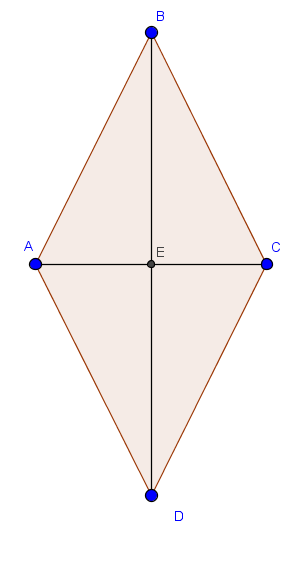
\includegraphics[scale=0.5]{./img/losa}
	\end{multicols}
			
	\end{myprops}


\subsection{Rectangle}

\begin{myprops}
	
	\begin{multicols}{2}
		
		Dans un rectangle :
		\begin{itemize}
			\item Les cotés opposés égaux;
			\item Les quatre angles sont des angles droits;
			\item Les diagonales se coupent en leur milieu et sont de même longueur;
			
		\end{itemize}
		
		
		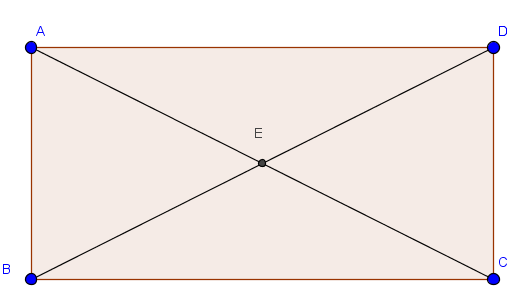
\includegraphics[scale=0.5]{./img/rect}
	\end{multicols}

\end{myprops}

\begin{mymeth}
		On calcule l'aire d'un rectangle en utilisant la formule suivante :
		\kw{\begin{align*}
			Aire &= Longueur \times  largeur
			\end{align*}}
		\vspace*{-1cm}
		\begin{align*}
		Aire &= AB \times AD
		\end{align*}
\end{mymeth}

\subsection{Carré}

\begin{myprops}
	
	\begin{multicols}{2}
		
		Dans un carré :
		\begin{itemize}
			\item Les quatre cotés sont égaux;
			\item Les quatre angles sont des angles droits;
			\item Les diagonales se coupent en perpendiculairement en leur milieu et sont de même longueur;
			
		\end{itemize}
		
		
		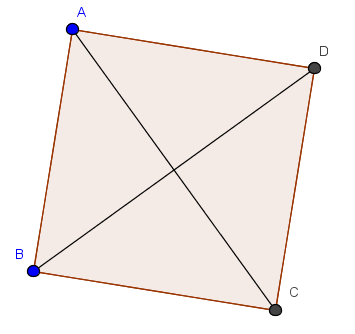
\includegraphics[scale=0.6]{./img/carre}
	\end{multicols}
	
\end{myprops}

\begin{mymeth}
	On calcule l'aire d'un carré en utilisant la formule suivante :
	\kw{\begin{align*}
		Aire &= coté \times  coté
		\end{align*}}
	\vspace*{-1cm}
	\begin{align*}
	Aire &= AB \times AB
	\end{align*}
\end{mymeth}

\section{Cercle et disque}

\begin{mymeth}
	\begin{multicols}{2}
		On calcule la circonférence d'un cercle en utilisant la formule suivante :
		\begin{align*}
			C &= 2\times \pi \times Rayon\\
			C &= 2\times \pi \times AB
		\end{align*}
		
		On calcule l'aire d'un disque en utilisant la formule suivante :
		\begin{align*}
		C &= \pi \times Rayon^2\\
		C &= \pi \times AB^2
		\end{align*}
		
		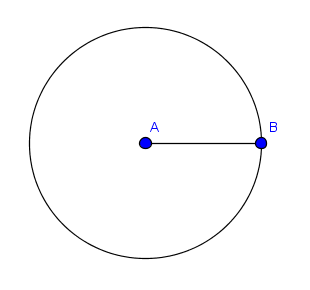
\includegraphics[scale=0.7]{img/cercle}
	\end{multicols}
\end{mymeth}
\end{document}